\documentclass{article}
\usepackage{polski}
\usepackage[utf8]{inputenc}
\usepackage{amsmath}
\usepackage{tikz}

\begin{document}

\title{Bazy Danych 2025 - Lista zadań nr 3}
\author{Artur Bieniek}

\maketitle

\section*{Rozgrzewka}
$P_7(x,y) \equiv \exists u \exists v P_3(x, u) \wedge P_2(u, v) \wedge P_2(v, y)$

\section{(1 pkt)}
Pokaż, że nie istnieje takie zapytanie koniunkcyjne używające jako formuł atomowych wyłącznie perspektyw $P_3(x, y)$ i $P_4(x, y)$, które jest równoważne zapytaniu $P_5(x, y)$.
\newline \textbf{Rozwiązanie:}
% To zapytanie w szczególności może zawierać tylko atomy $P_3(x, y)$ i $P_4(x, y)$ oraz koniunkcje i kwantyfikatory egzystencjalne.
% Musi więc ono być postaci $\exists u P_i(x, u) \wedge P_{5-i}(u, y)$ dla $i \in \{1, 2, 3, 4\}$. Ale zauważmy że $5-3 = 2$ oraz $5-4 = 1$, a nie możemy wykorzystać $P_1$ ani $P_2$, więc takiego zapytania nie można skonstruować.
$P_5(x, y)$ oznacza że istnieje ścieżka długości $5$ z $x$ do $y$. Czyli istnieje ciąg wierzchołków $x, v_1, v_2, v_3, v_4, y$ połączonych kolejno krawędziami. Za pomocą zapytania składającego się tylko i wyłącznie z perspektyw $P_3(x, y)$ oraz $P_4(x, y)$, kwantyfikatorów egzystencjalnych i operatora koniunkcji jesteśmy w stanie sprawdzić tylko czy istnieją $v_1, v_2, v_3, v_4$ spełniające następujące własności:
\begin{itemize}
        \item $P_3(x, v_3)$
        \item $P_3(v_1, v_4)$
        \item $P_3(v_2, y)$
        \item $P_4(x, v_4)$
        \item $P_4(v_1, y)$
\end{itemize}
Teraz pokażemy graf który nie zawiera ścieżki długości $5$ z $x$ do $y$ (właściwie nie zawiera nawet żadnej ścieżki z $x$ do $y$), a spełnia wszystkie te własności.
\newline
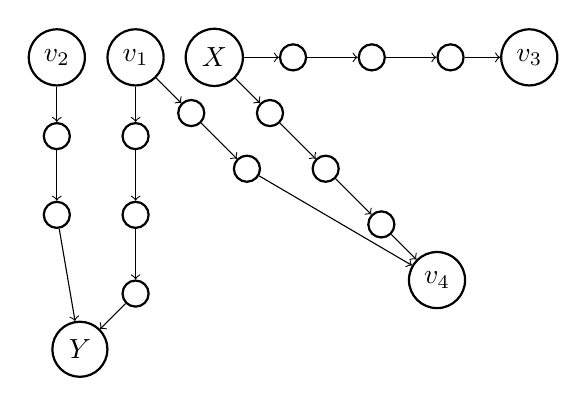
\begin{tikzpicture}[main/.style = {thick, draw, circle}] 
        \node[main] (1) {$v_2$};
        \node[main] (2) [right of=1] {$v_1$};
        \node[main] (3) [right of=2] {$X$};
        \node[main] (4) [right of=3] {};
        \node[main] (5) [right of=4] {};
        \node[main] (6) [right of=5] {};
        \node[main] (7) [right of=6] {$v_3$};
        \node[main] (8) [below right of=3] {};
        \node[main] (9) [below right of=8] {};
        \node[main] (10) [below right of=9] {};
        \node[main] (11) [below right of=10] {$v_4$};
        \node[main] (12) [below right of=2] {};
        \node[main] (13) [below right of=12] {};
        \node[main] (14) [below of=2] {};
        \node[main] (15) [below of=14] {};
        \node[main] (16) [below of=15] {};
        \node[main] (17) [below left of=16] {$Y$};
        \node[main] (18) [below of=1] {};
        \node[main] (19) [below of=18] {};

        \draw[->] (1) -- (18);
        \draw[->] (18) -- (19);
        \draw[->] (19) -- (17);

        \draw[->] (2) -- (14);
        \draw[->] (14) -- (15);
        \draw[->] (15) -- (16);
        \draw[->] (16) -- (17);

        \draw[->] (2) -- (12);
        \draw[->] (12) -- (13);
        \draw[->] (13) -- (11);

        \draw[->] (3) -- (8);
        \draw[->] (8) -- (9);
        \draw[->] (9) -- (10);
        \draw[->] (10) -- (11);

        \draw[->] (3) -- (4);
        \draw[->] (4) -- (5);
        \draw[->] (5) -- (6);
        \draw[->] (6) -- (7);
\end{tikzpicture}
\newline
Przypuśćmy że mamy reprezentację $P_5(x, y)$. Zauważmy jednak że względem niej istnieje homomorfizm grafu w wyżej przedstawiony graf, dla którego zapytanie zwraca błędny wynik.

\section{(1 pkt)}
Napisz zapytanie rrd (dozwolone $\exists, \forall$ i wszystkie spójniki boolowskie), które korzysta wyłącznie z perspektyw $P_3(x, y)$ i $P_4(x, y)$ i jest równoważne zapytaniu $P_5(x, y)$.
\newline \textbf{Rozwiązanie:}
$P_5(x,y) \equiv 
\exists v_4 [P_4(x, v_4) \wedge \forall v_1 (P_3(v_1, v_4) \implies P_4(v_1, y))]
$
\newline Dlaczego to działa?
Weźmy dowolny wierzchołek $v_4$, do którego można dojść ścieżką długości $4$ z $x$. Weźmy teraz wszystkie takie wierzchołki $v_1$, z których można dojść do $v_4$ ścieżką długości $3$. Zauważmy, że jest wśród nich pierwszy wierzchołek na ścieżce z $x$ do $v_4$. Jeśli z wszystkich takich wierzchołków można dojść do $y$ ścieżką długości $4$, to w szczególności można dojść z $x$ do $y$ ścieżką długości $5$.
\newline \newline
Jeśli nie istnieje wierzchołek, do którego można dojść ścieżką długości $4$ z $x$, to w szczególności nie istnieje też taki do którego można dojść ścieżką długości $5$ z $x$.
\newline
Jeśli zaś istnieje wierzchołek taki, że można z niego dojść do $v_4$ ścieżką długości $4$, ale nie można dojść z niego do $y$ ścieżką długości $5$, to w szczególności oznacza to, że ścieżki do $v_4$ nie można przedłużyć o krawędź z $v_4$ do $y$, więc ta krawędź nie istnieje.

\section{(1 pkt)}
\begin{enumerate}
        \item Pokaż, że istnieje graf $G$, taki, że dla dowolnego grafu $G'$ istnieje homomorfizm z $G'$ w $G$.
        \newline \textbf{Rozwiązanie:}
        Weźmy graf $G(V, E)$, gdzie $V={v_1}$, $E=\{(v_1, v_1)\}$, czyli po prostu graf który ma pojedynczy wierzchołek i pętelkę. Weźmy teraz dowolny graf $G'(V', E')$. Zdefiniujmy homomorfizm $h : V' \rightarrow V$ taki, że $\forall v \in V' h(v) = v_1$, czyli przekształcamy wszystkie wierzchołki na wierzchołek $v_1$. Weźmy dowolną krawędź $(u, v) \in E'$. Zauważmy, że $(h(u), h(v)) = (v_1, v_1) \in E$. Czyli pokazaliśmy taki graf $G$, że dla dowolnego grafu $G'$ istnieje homomorfizm z $G'$ w $G$.

        \item Udowodnij lub podaj kontrprzykład na stwierdzenie: dla dowolnych grafów $G_1$ i $G_2$ następujące warunki są równoważne:
        \begin{itemize}
                \item istnieją homomorfizmy $h_1 : G_1 \rightarrow G_2$ oraz $h_2 : G_2 \rightarrow G_1$ (mówimy, że takie grafy są \textit{homomorficznie równoważne})
                \item istnieje izomorfizm- $f : G_1 \rightarrow G_2$
        \end{itemize}
        \textbf{Rozwiązanie:} Weźmy następujące grafy: \newline
        $G_1(\{u_1, u_2\}, \{(u_1, u_1), (u_1, u_2)\})$ i $G_2(\{v_1\}, \{(v_1, v_1)\})$
        \newline Istnieje homomorfizm $h_1 : G_1 \rightarrow G_2$, taki że
        $\forall v \in V_1 h_1(v)=v_1$.
        \newline Istnieje homomorfizm $h_2 : G_2 \rightarrow G_1$, taki że
        $\forall v \in V_2 h_2(v)=u_1$.
        \newline Ale nie istnieje izomorfizm $G_1 \rightarrow G_2$, ponieważ izomorfizm w szczególności jest bijekcją, a nie można zrobić bijekcji między zbiorami, które nie są równoliczne.
\end{enumerate}

\section{(1 pkt)}
W tym zadaniu rozważamy grafy symetryczne tzn. takie, że jeśli istnieje krawędź z $v$ do $w$ to istnieje też krawędź z $w$ do $v$. Pokaż, że każde dwa takie grafy będące cyklami o parzystej długości są homomorficznie równoważne.
\newline \textbf{Rozwiązanie:} Bez straty ogólności pokażemy homomorfizm $G_1 \rightarrow G_2$. Skoro grafy te są cyklami parzystej długości, to są one dwudzielne, czyli dwukolorowalne, czyli istnieje z nich homomorfizm w $K_2$ (równoważność tych rzeczy była pokazywana na wykładzie). Zauważmy, że jeśli weźmiemy (dowolne) dwa wierzchołki połączone krawędzią z $G_2$, to otrzymamy graf $K_2$. Skoro istnieje homomorfizm $G_1 \rightarrow K_2$ oraz $G_2$ zawiera $K_2$, to istnieje homomorfizm $G_1 \rightarrow G_2$.

\section{(1 pkt)}
Mówimy, że formuła rachunku zdań jest w postaci 3CNF, gdy jest w koniunkcyjnej postaci normalnej, a dodatkowo każda klazula zawiera najwyżej 3 zmienne. Przykład formuły 3CNF: $(p \vee \neg q \vee r) \wedge (s \vee \neg r)$.
Rozważmy problem spełnialności formuł rachunku zdań zwany 3SAT: dla danej formuły w postaci 3CNF, rozstrzygnij czy istnieje wartościowanie ją spełniające.
Pokaż, że problem 3SAT można wyrazić jako problem istnienia homomorfizmu pomiędzy bazami danych, tzn. pokaż, że jesli potrafisz rozwiązywać problem istnienia homomorfizmu to potrafisz także rozwiązywać problem 3SAT. Twoja konstrukcja powinna działać w czasie wielomianowym.
\newline \textbf{Rozwiązanie:}
Skonstruujmy relacje:
\begin{itemize}
        \item $V_1 = \{\{T, F\}, \{F, T\}\}$
        \item $V_2 = \{ 
                \{ T, T, T \},
                \{ T, T, F \},
                \{ T, F, T \},
                \{ T, F, F \},
                \{ F, T, T \},
                \{ F, T, F \},
                \{ F, F, T \}
                \}$.
        \item $F_1$ taką że $(p, \neg p) \in F_1 \iff p$ występuje w zapytaniu.
        \item $F_2$ taką że $(p, q, r) \in F_2 \iff (p \vee q \vee r)$ występuje w formule 3CNF, przy czym $p, q, r$ mogą zawierać negacje, a jeśli w formule 3CNF występuje człon w którym jest tylko alternatywa 1 lub 2 elementów, to ostatni element powtarzamy odpowiednio 2 razy lub 1 raz.
\end{itemize}
Teraz jeśli istnieje homomorfizm $F_1 \rightarrow V_1$ oraz istnieje homomorfizm $F_2 \rightarrow V_2$, to podana formuła 3CNF jest spełnialna, ponieważ homomorfizm ten przyporządkował zmiennym wartościowania w taki sposób, że każdy człon formuły 3CNF jest spełniony, ponieważ w relacji $V_2$ nie ma krotek z 3 fałszami, a tylko wtedy alternatywa może być fałszem.

\section{(0.5 pkt)}
Wiadomo, że problem 3SAT jest trudny obliczeniowo. Za wykazanie, że istnieje jakikolwiek wielomianowy algorytm rozwiązujący ten problem Clay Institute ufundował nagrodę w wysokości miliona dolarów. Problem ewaluacji zapytań koniunkcyjnych (czyli istnienia homomorfizmu) nie jest uznawany za szczególnie trudny, a silniki bazodanowe od wielu lat wydajnie wyliczają odpowiedzi na zapytania SQL. Tymczasem w zadaniu 5 tak naprawdę pokazaliśmy, że problem 3SAT jest łatwiejszy (lub równie trudny) jak problem istnienia homomorfizmu. Wyjaśnij dlaczego to nie jest paradoks (a rozwiązanie zadania 5 nie wystarczy
aby otrzymać nagrodę).
\newline \textbf{Rozwiązanie:}
Silniki bazodanowe wydajnie wyliczają odpowiedzi na zapytania koniunkcyjne, ponieważ w praktyce są one stosunkowo proste. Zauważmy, że algorytmem o złożoności wykładniczej można bez problemu na dzisiejszych komputerach w czasie poniżej sekundy rozwiązać problem 3SAT dla 20 różnych zmiennych, ponieważ wymaga to jedynie sprawdzenia $2^{20} \approx 10^7$ różnych wartościowań. W praktyce zapytanie koniunkcyjne składające się z 20 różnych zmiennych jest już uważane za bardzo skomplikowane.

\section{(0.5 pkt)}
Zaproponuj algorytm obliczania dla danej bazy ze zmiennymi $D$ zbioru
\[
        \bigcap\{I \mid I \in rep(D)\}
\]
tzn. zbioru krotek obecnych w każdej bazie w $rep(D)$, zbiór ten oznaczmy $sure(D)$.
Z jakich krotek składa się ten zbiór?
\newline \textbf{Rozwiązanie:}
Zauważmy, że krotka $k$ należy do tego zbioru wtw, gdy każda wartość z krotki $k$ jest identyczna w każdej reprezentacji bazy danych $D$. Wynika stąd, że do tego zbioru należą te krotki z bazy $D$, które nie zawierają zmiennych. Czyli algorytm wyznaczania takiego zbioru przechodzi po krotkach relacji i bierze te krotki w których nie występują zmienne.

\section{(0.5 pkt)}
Rozważmy następującą definicję wyniku zapytania
\[
        Q_D = sure(Q, D)
\]
Zauważ, że to nie jest dobra definicja. Skonstruuj relację D i dwa zapytania $Q'$ i $Q''$ takie, że obliczenie wyniku zapytania $Q'' \circ Q'$ będącego złożeniem $Q''$ i $Q'$ na D zwraca inną odpowiedź niż obliczenie $Q''$ na $sure(Q', D)$ czyli na bazie będącej wynikiem obliczenia $Q'$ na $D$. Zapisując formalnie:
\[
        sure(Q'' \circ Q', D) \neq sure(Q'', sure(Q', D))
\]
W naszym przypadku złożenie zapytania $Q''$ i $Q'$ to po prostu wyrażenie algebry relacji $Q''$, w którym wszystkie odwołania do bazy wejściowej zastąpiono wyrażeniem $Q'$. Np. złożeniem zapytań $\sigma_{B=C} (D)$ i $\sigma_{A>7}(D)$ jest wyrażenie $\sigma_{B=C} (\sigma_{A>7}(D))$.
\newline Hint: szukaj prostego tricku - o czym zapominamy biorąc jako wynik pośredni $sure(Q', D)$?

\textbf{Rozwiązanie:}
Weźmy relację $D = \{ (1,X) \}$, o schemacie A,B.
Niech $Q' = \sigma_{A=1}(D)$, $Q'' = \pi_{A}(D)$.
Wtedy $sure(Q', D) = \emptyset$, $sure(Q'', sure(Q', D)) = \emptyset$, $sure(Q'' \circ Q', D) = \{ (1) \}$.
\newline \textbf{Wniosek:} wynik $Q_D$ trzeba zdefiniować tak aby zawierał więcej informacji niż $sure(Q, D)$.

\section{(1 pkt, nie wlicza się do maksimum)}
Przetestujmy więc kolejne podejście. Tym razem na $Q_D$ zamiast warunku
\[
        rep(Q_D) = Q(rep(D))
\]
nałożmy taki:
\[
        sure(Q_D) = sure(Q, D)
\]
Czyli wymagamy aby zbiór krotek w przekroju wszystkich baz z $rep(Q_D)$ był równy $sure(Q, D)$. Różnica w stosunku do poprzedniego podpunktu jest teraz taka, że nasz wynik $Q_D$ może zawierać krotki ze zmiennymi. Pokaż jak zdefiniować selekcję oraz projekcję na bazach z zmiennymi tak aby dla dowolnego zapytania $Q$ zbudowanego z selekcji i projekcji oraz dowolnej bazy ze zmiennymi $D$ wynik $Q_D$ istniał, spełniał warunek
\[
        sure(Q_D) = sure(Q, D)
\]
, a dodatkowo zapytania można było składać.
\newline \textbf{Rozwiązanie:}
Zdefiniujmy selekcję w następujący sposób (dla uproszczenia tylko z jednym termem, selekcję z wieloma termami można uzyskać przez złożenie wielu selekcji z jednym termem):
\[
        \sigma_{K=v}(D) = \{ k \in D \mid k.K=v \}
\]
Oznacza to, że krotki zawierające zmienne mogą znaleźć się w wyniku selekcji wtw, gdy te zmienne nie były w warunkach selekcji.
Projekcję definiujemy w identyczny sposób jak jest ona zdefiniowana dla relacji bez zmiennych, czyli po prostu wybieramy kolumny, nie ma znaczenia czy krotki mają na tych kolumnach zmienne czy też nie.
\newline
Nie gubimy więc informacji o zmiennych, po których nie zrobiliśmy selekcji.
\end{document}